% !TeX root = origami-math-he.tex

\selectlanguage{hebrew}
\appendix


\chapter{קישוריות לגיאוגברה}\label{a.geo}

\begin{center}
\begin{tabular}{|l|l|}
\hline
$1$ \R{אקסיומה}& \url{https://www.geogebra.org/m/fq9d5hms}\\\hline
$2$ \R{אקסיומה}& \url{https://www.geogebra.org/m/fgmfss27}\\\hline
$3$ \R{אקסיומה}& \url{https://www.geogebra.org/m/ek3mqupw}\\\hline
$4$ \R{אקסיומה}& \url{https://www.geogebra.org/m/renzzbdg}\\\hline
$5$ \R{אקסיומה}& \url{https://www.geogebra.org/m/aszn9ywu}\\\hline
$6$ \R{אקסיומה}& \url{https://www.geogebra.org/m/bxe5e5ku}\\\hline
$7$ \R{אקסיומה}& \url{https://www.geogebra.org/m/yeq5gmeg}\\\hline
Abe \R{חקלוקת זווית לשלושה של} & \url{https://www.geogebra.org/m/dxrcvjam}\\\hline
Martin \R{חקלוקת זווית לשלושה של}& \url{https://www.geogebra.org/m/caky7edd}\\\hline
Messer \R{הכפלת קוביה של} & \url{https://www.geogebra.org/m/mrcwjqh8}\\\hline
Beloch \R{הכפלת קוביה של}  & \url{https://www.geogebra.org/m/enzmmwua}\\\hline
\end{tabular}
\end{center}
לאור תקלה בגיאוגברה, בפרוייקטים המשתמשים באקסיומה $6$, נקודות המוגדרות על ידי שיקוף מסביב למשיק המשותף אינן נשמרות או נשמרות בצורה שגוייה.

\chapter{פיתוח הזהיות הטריגונומטריות}\label{a.tangent}

ניתן לפתח את הזהויות הטריגונומטריות עבור טנגנס שהשתמשנו בהוכחה של אקסיומה~$3$ מזהויות עבור סינוס וקסינוס:

\begin{form}{2.2}
\tan (\theta_1+\theta_2) &=& \disfrac{\sin(\theta_1+\theta_2)}{\cos(\theta_1+\theta_2)}\\
&=&\disfrac{\sin\theta_1\cos\theta_2+\cos\theta_1\sin\theta_2}{\cos\theta_1\cos\theta_2-\sin\theta_1\sin\theta_2}\\
&=&\disfrac{\sin\theta_1+\cos\theta_1\tan\theta_2}{\cos\theta_1-\sin\theta_1\tan\theta_2}\\
&=&\disfrac{\tan\theta_1+\tan\theta_2}{1-\tan\theta_1\tan\theta_2}\,.
\end{form}
נשמתש משוואה זו עם
$\theta=(\theta/2)+(\theta/2)$
ונקבל משוואה ריבועית במשתנה
$\tan(\theta/2)$:
\begin{form}{2.2}
\tan \theta=\disfrac{\tan(\theta/2)+\tan(\theta/2)}{1-\tan^2(\theta/2)}\\
\tan\theta \,(\tan(\theta/2))^2 \;+\; 2\,(\tan (\theta/2)) \;-\;\tan \theta = 0\,.
\end{form}
הפתרונות שלה הם:
\[
\tan(\theta/2) = \disfrac{-1\pm\sqrt{1+\tan^2\theta}}{\tan\theta}\,.
\]


\chapter{פרבולות}\label{a.parabola}

בתחילת דרכם, תלמידים מכירים פרבולות כגרפים של פולינומים ריבועיים
$y=ax^2+bx+c$.
אולם ניתן הגדיר פרבולות באמצעות גיאומטריה: נתונה נקודה, 
\textbf{המוקד} \L{(focus)},
ונתון קו,
\textbf{המדריך} \L{(directrix)},
המקום הגיאומטרי של הנקודות הנמצאות במרחק שווה מהמוקד ומהמדריך מגדיר פרבולה.

האיור שלהלן מראה את המוקד -- הנקודה הגדולה ב-%
$p=(0,f)$, 
והמדריך -- הקו העבה עם המשוואה
$y=-f$. 
הפרבולה המתקבלת מוצגת בקו מנוקד. 
\textbf{הקודקוד} \L{(vertex)}
שלה 
$p_2$
נמצא במרכז הצירים.
\begin{center}
\selectlanguage{english}
\begin{tikzpicture}[scale=1]
\draw (-6,0) -- node[very near start,below,xshift=-32pt] {$x$-\textsf{axis}} (6,0);
\draw (0,-3) -- node[very near start,right,yshift=-20pt] {$y$-\textsf{axis}} (0,4.5);
\draw[ultra thick] (-6,-2) -- node[near end,below] {\textsf{directrix} $d: \quad y=-f$} (6,-2);
\draw[domain=-6:6,samples=50,very thick,dotted] plot (\x,{\x*\x/8});
\coordinate (F) at (0,2);
\fill (F) circle (3pt) node[above left,xshift=-2pt,yshift=15pt] {$(0,f)$} node[above left,xshift=-2pt,yshift=30pt] {\textsf{focus}} node[above right] {$p$};
\fill (0,0) circle (1.5pt) node[below right] {$p_2$};
\fill (0,-2) circle (1.5pt);
\fill (2,-2) circle (1.5pt);
\fill (3,-2) circle (1.5pt);
\fill (5,-2) circle (1.5pt);
\coordinate (FP) at (-5,-2);
\fill (FP) circle (1.5pt) node[below] {$p_1'$};
\coordinate (F1) at (2,.5);
\fill (F1) circle (1.5pt) node[below right] {$p_3$};
\coordinate (F2) at (3,1.125);
\fill (F2) circle (1.5pt) node[below right] {$p_4$};
\coordinate (F3) at (5,3.125);
\fill (F3) circle (1.5pt) node[below right] {$p_5$};
\coordinate (F4) at (-5,3.125);
\fill (F4) circle (1.5pt) node[above right] {$p_1$};
\draw (F) -- node[left] {$a_2$} (0,0) -- node[left] {$a_2$} (0,-2);
\draw (F) -- node[near end,left] {$a_3$} (F1) -- node[left] {$a_3$} (2,-2);
\draw (F) -- node[near end,above] {$a_4$} (F2) -- node[left] {$a_4$} (3,-2);
\draw (F) -- node[above] {$a_5$} (F3) -- node[left] {$a_5$} (5,-2);
\draw (F) -- node[above] {$a_1$} (F4) -- node[left] {$a_1$} (FP);
\draw[thick,dashed] ($(F4)!-.4!(-2.5,0)$) -- node[very near end,right,xshift=2pt] {$l_1$} ($(F4)!1.8!(-2.5,0)$);
\draw (0,-2) rectangle +(8pt,8pt);
\draw (2,-2) rectangle +(8pt,8pt);
\draw (3,-2) rectangle +(8pt,8pt);
\draw (5,-2) rectangle +(8pt,8pt);
\draw (-5,-2) rectangle +(8pt,8pt);
\end{tikzpicture}
\end{center}

בחרנו חמש נקודות
$p_i$, $i=1,\ldots,5$
על הפרבולה. כל נקודה
$p_i$
הוא במרחק
$a_i$
גם מהמוקד וגם מהמדריך. נוריד ניצב למדריך מ-%
$p_i$,
ונסמן ב-%
$p_i'$
את נקודת החיתוך של הניצב עם המדריך. נשתמש באקסיומה $2$ ונבנה את הקו 
$l_i$
דרך
$p_i$
שמשקף את 
$p$
על
$p_i'$.
האיור מראה את הקיפול 
$l_1$
דרך 
$p_1$.

\newpage

\textbf{משפט}
הקיפולים הם משיקים לפרבולה.

\textbf{הוכחה )אוריה בן לולו(}
באיור שלהלן, המוקד הוא 
$p$,
המדריך הוא 
$l$,
$p'$
היא נקודה על המדריך, ו-%
$m$
הוא הקיפול המשקף את
$p$
על 
$p'$.
לפי ההגדרה, 
$m$
הוא האנך האמצעי של הקו
$\overline{pp'}$.
תהי 
$s$
החיתוך של 
$\overline{pp'}$
ו-%
$m$;
אזי 
$\overline{ps}=\overline{p's}=a$
ו-%
$m\perp \overline{pp'}$.

\begin{center}
\selectlanguage{english}
\begin{tikzpicture}[scale=1.1]
\draw[ultra thick] (-6,-2) -- node[near end, below] {$l$} (6,-2);
\draw[domain=-5.5:5.5,samples=50,very thick,dotted] plot (\x,{\x*\x/8});
\coordinate (F) at (0,2);
\fill (F) circle (2pt) node[above right] {$p$};
\coordinate (FP) at (-3,-2);
\fill (FP) circle (1.5pt) node[below] {$p'$};
\coordinate (F4) at (-3,1.125);
\fill (F4) circle (1.5pt) node[above right] {$r$};
\coordinate (F5) at (-5,2.775);
\fill (F5) circle (1.5pt) node[left,yshift=-4pt] {$q$};
\coordinate (F5p) at (-5,-2);
\fill (F5p) circle (1.5pt) node[below] {$p''$};
\draw (F) -- node[above] {$b$} (F4) -- node[left] {$b$} (FP);
\draw (F) -- node[above] {$c$} (F5);
\draw (F5) -- node[left] {$d$} (F5p);
\draw[thick,dashed,name path=fold] ($(F4)+(140:4)$) -- (F4) -- node[below,xshift=-2pt,yshift=-2pt] {$m$} ($(F4)+(-40:5.1)$);
\draw (FP) rectangle +(8pt,8pt);
\draw (F5p) rectangle +(8pt,8pt);
\draw (F5) -- (FP);
\draw[name path=base] (F) -- (FP);
\path [name intersections = {of = base and fold, by = {G}}];
\fill (G) circle (1.5pt) node[below,yshift=-4pt] {$s$};
\draw[rotate=140] (G) rectangle +(6pt,6pt);
\path (FP) -- node[left] {$c$} (F5);
\path (F) -- node[below] {$a$} (G) -- node[below] {$a$} (FP);
\end{tikzpicture}
\end{center}

תהי
$r$
החיתוך של הניצב ל-%
$l$
דרך 
$p'$
והקיפול
$m$.
אזי
$\triangle psr\cong \triangle p'sr$
לפי צלע-זווית-צלע, כי
$\overline{ps}=\overline{p's}$, 
$\angle psr=\angle p'sr=90^\circ$
ו-%
$\overline{rs}$
הוא צלע משותפת. מכאן ש-%
$\overline{pr}=\overline{p'r}=b$
ולכן
$r$
נמצאת על הפרבולה.

בחר נקודה
$p''$
על המדריך שהיא שונה מ-%
$p'$,
והנח שהקיפול
$m$
גם משקף את
$p$ 
על
$p''$.
תהי 
$q$
החיתוך של הניצב ל-%
$l$
דרך 
$p''$
והקיפול
$m$.
כמו בהוכחה לעיל, נוכל להוכיח ש-%
$\overline{pq}=\overline{p'q}=c$.
נסמן
$\overline{qp''}=d$.
אם
$q$
נמצאת על הפרבולה, אזי
$d=\overline{qp''}=\overline{qp}=c$.
אבל
$c$
הוא היתר של המשולש ישר-זווית
$\triangle qp''p'$
ולא יכול להיות שווה לאחד הצלעות שלו
$d$.

הוכחנו של-%
$m$
נקודת חיתוך אחד עם בפרבולה ולכן הוא משיק לפרבולה.


\chapter{משיקים המשותפים לשתי פרבולות}\label{a.number-of-tangents}

להלן איורים המדגימים את ארבעת האפשרויות:

\bigskip\bigskip

\begin{center}
\selectlanguage{english}
\begin{tikzpicture}[scale=.8]
\draw (-7,0) -- (7,0);
\draw (0,-1) -- (0,7);
\coordinate (P1) at (0,6);
\fill (P1) circle (2pt) node[above left] {$p_1$};
\coordinate (P2) at (0,2);
\fill (P2) circle (2pt) node[above left] {$p_2$};
\draw[thick] (-7,3) -- node[very near start,above,xshift=-25pt] {$l_1$} (7,3);
\draw[thick] (-7,1) -- node[very near start,above,xshift=-25pt] {$l_2$} (7,1);
\draw[domain=-3.1:3.1,samples=50,very thick,dotted] plot (\x,{.25*\x*\x+4.5});
\draw[domain=-4.5:4.5,samples=50,very thick,dotted] plot (\x,{.25*\x*\x+1.5});
\end{tikzpicture}
\end{center}

\bigskip\bigskip

\begin{center}
\selectlanguage{english}
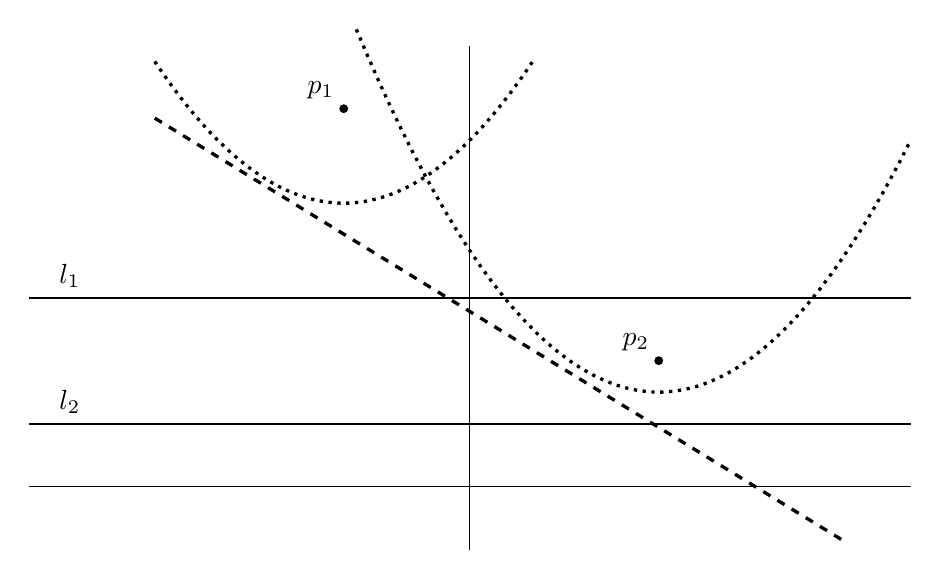
\begin{tikzpicture}[scale=.8]
\draw (-7,0) -- (7,0);
\draw (0,-1) -- (0,7);
\coordinate (P1) at (-2,6);
\fill (P1) circle (2pt) node[above left] {$p_1$};
\coordinate (P2) at (3,2);
\fill (P2) circle (2pt) node[above left] {$p_2$};
\draw[thick] (-7,3) -- node[very near start,above,xshift=-25pt] {$l_1$} (7,3);
\draw[thick] (-7,1) -- node[very near start,above,xshift=-25pt] {$l_2$} (7,1);
\draw[domain=-5:1,samples=50,very thick,dotted] plot (\x,{.25*(\x+2)*(\x+2)+4.5});
\draw[domain=-1.8:7,samples=50,very thick,dotted] plot (\x,{.25*(\x-3)*(\x-3)+1.5});
\draw[very thick,dashed] (-5,5.85) -- (6,-.9);
\end{tikzpicture}
\end{center}

\bigskip\bigskip

\begin{center}
\selectlanguage{english}
\begin{tikzpicture}[scale=.8]
\draw (-7,0) -- (7,0);
\draw (0,-7) -- (0,5);
\coordinate (P1) at (0,4);
\fill (P1) circle (2pt) node[above left] {$p_1$};
\coordinate (P2) at (0,-6);
\fill (P2) circle (2pt) node[above left] {$p_2$};
\draw[thick] (-7,2) -- node[very near start,above,xshift=-25pt] {$l_1$} (7,2);
\draw[thick] (-7,-2) -- node[very near start,below,xshift=-25pt] {$l_2$} (7,-2);
\draw[domain=-4.8:4.8,samples=50,very thick,dotted] plot (\x,{-.13*\x*\x-4});
\draw[domain=-2.8:2.8,samples=50,very thick,dotted] plot (\x,{.25*\x*\x+3});
\draw[very thick,dashed] (-5,-7) -- (2.95,5);
\draw[very thick,dashed] (-3,5) -- (4.95,-7);
\end{tikzpicture}
\end{center}

\bigskip\bigskip

\begin{center}
\selectlanguage{english}
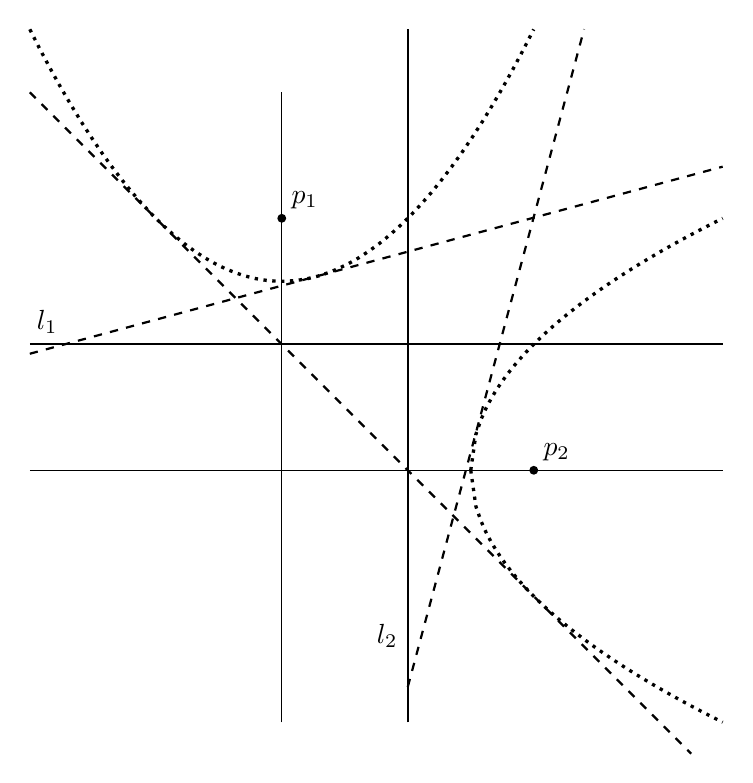
\begin{tikzpicture}[scale=.8]
\draw (-4,0) -- (7,0);
\draw (0,-4) -- (0,6);
\coordinate (P1) at (0,4);
\fill (P1) circle (2pt) node[above right] {$p_1$};
\coordinate (P2) at (4,0);
\fill (P2) circle (2pt) node[above right] {$p_2$};
\draw[thick] (-4,2) -- node[very near start,above,xshift=-25pt] {$l_1$} (7,2);
\draw[thick] (2,-4) -- node[very near start,left] {$l_2$} (2,7);
\draw[domain=-4:4,samples=50,very thick,dotted] plot (\x,{.25*\x*\x+3});
\draw[domain=3:7,samples=50,very thick,dotted] plot (\x,{sqrt(4*\x-12)});
\draw[domain=3:7,samples=50,very thick,dotted] plot (\x,{-sqrt(4*\x-12)});

\draw[thick,dashed,domain=-4:6.5] plot (\x,-\x+2);
\draw[thick,dashed,domain=-4:7] plot (\x,.27*\x+2.93);
\draw[thick,dashed,domain=2:4.8] plot (\x,3.73*\x-10.9);
\end{tikzpicture}
\end{center}

